%% abtex2-modelo-trabalho-academico.tex, v<VERSION> laurocesar
%% Copyright 2012-<COPYRIGHT_YEAR> by abnTeX2 group at http://www.abntex.net.br/ 
%%
%% This work may be distributed and/or modified under the
%% conditions of the LaTeX Project Public License, either version 1.3
%% of this license or (at your option) any later version.
%% The latest version of this license is in
%%   http://www.latex-project.org/lppl.txt
%% and version 1.3 or later is part of all distributions of LaTeX
%% version 2005/12/01 or later.
%%
%% This work has the LPPL maintenance status `maintained'.
%% 
%% The Current Maintainer of this work is the abnTeX2 team, led
%% by Lauro César Araujo. Further information are available on 
%% http://www.abntex.net.br/
%%
%% This work consists of the files abntex2-modelo-trabalho-academico.tex,
%% abntex2-modelo-include-comandos and abntex2-modelo-references.bib
%%

% ------------------------------------------------------------------------
% ------------------------------------------------------------------------
% abnTeX2: Modelo de Trabalho Academico (tese de doutorado, dissertacao de
% mestrado e trabalhos monograficos em geral) em conformidade com 
% ABNT NBR 14724:2011: Informacao e documentacao - Trabalhos academicos -
% Apresentacao
% ------------------------------------------------------------------------
% ------------------------------------------------------------------------

\documentclass[
	% -- opções da classe memoir --
	12pt,				% tamanho da fonte
	openright,			% capítulos começam em pág ímpar (insere página vazia caso preciso)
	twoside,			% para impressão em recto e verso. Oposto a oneside
	a4paper,			% tamanho do papel. 
	% -- opções da classe abntex2 --
	%chapter=TITLE,		% títulos de capítulos convertidos em letras maiúsculas
	%section=TITLE,		% títulos de seções convertidos em letras maiúsculas
	%subsection=TITLE,	% títulos de subseções convertidos em letras maiúsculas
	%subsubsection=TITLE,% títulos de subsubseções convertidos em letras maiúsculas
	% -- opções do pacote babel --
	english,			% idioma adicional para hifenização
	french,				% idioma adicional para hifenização
	spanish,			% idioma adicional para hifenização
	brazil,				% o último idioma é o principal do documento
	sumario=tradicional
	]{abntex2}

% ---
% Carregando pacotes necessários para gerar o PDF 
% ---
% ---
% Pacotes básicos 
% ---
\usepackage{lmodern}		% Usa a fonte Latin Modern			
\usepackage[T1]{fontenc}	% Selecao de codigos de fonte.
\usepackage[utf8]{inputenc}	% Codificacao do documento (conversão automática dos acentos)
\usepackage{lastpage}		% Usado pela Ficha catalográfica
\usepackage{indentfirst}	% Indenta o primeiro parágrafo de cada seção.
\usepackage{color}			% Controle das cores
\usepackage{xcolor}			% Controle das cores
\usepackage{graphicx}		% Inclusão de gráficos
\usepackage{microtype} 		% para melhorias de justificação
% ---
% Adicionado por Madson Dias
% ---

\graphicspath{ {figuras/graficos/} {figuras/imagens/}}  % Inclusão dos paths para imagens
\usepackage{xstring} 	% Criar comandos com IF
\usepackage{caption}
\usepackage{subcaption}
\usepackage{mdframed}
\usepackage{microtype}
\usepackage{pdfpages}
\usepackage{listings}
\usepackage{textcomp}
\usepackage{float}
\usepackage{chngcntr}		% Criar numeração de imagens por capítulo
\counterwithin{figure}{section}
\usepackage[os=win]{menukeys}
\usepackage{multicol}
\usepackage{framed}
% \usepackage{helvet}
% \usepackage{geometry}
% \usepackage{marginnote}

% ---
% Pacotes adicionais, usados apenas no âmbito do Modelo Canônico do abnteX2
% ---
\usepackage{lipsum}				% para geração de dummy text
% ---

% ---
% Pacotes de citações
% ---
\usepackage[brazilian,hyperpageref]{backref}	 % Paginas com as citações na bibl
\usepackage[alf]{abntex2cite}	% Citações padrão ABNT

% --- 
% CONFIGURAÇÕES DE PACOTES
% --- 

% ---
% Configurações do pacote backref
% Usado sem a opção hyperpageref de backref
\renewcommand{\backrefpagesname}{Citado na(s) página(s):~}
% Texto padrão antes do número das páginas
\renewcommand{\backref}{}
% Define os textos da citação
\renewcommand*{\backrefalt}[4]{
	\ifcase #1 %
		Nenhuma citação no texto.%
	\or
		Citado na página #2.%
	\else
		Citado #1 vezes nas páginas #2.%
	\fi}%
% ---

% ---
% Alterando espaçamento dos itens
% ---
\setlist[itemize]{noitemsep, topsep=0pt, leftmargin=1.75cm}
\setlist[enumerate]{noitemsep, topsep=0pt, leftmargin=1.75cm}
\setlist[description]{noitemsep, topsep=0pt, leftmargin=1.75cm}

% ---
% Alterando o aspecto da cor azul
% ---
\definecolor{blue}{RGB}{41,5,195}

% --- 
% Espaçamentos entre linhas e parágrafos 
% --- 

% O tamanho do parágrafo é dado por:
\setlength{\parindent}{1.3cm}

% Controle do espaçamento entre um parágrafo e outro:
\setlength{\parskip}{0.2cm}  % tente também \onelineskip

\usepackage{utils/ejovem-modelo} 	% Pacote com informações da customização
\usepackage{utils/ejovem-programacao-web} 	% Pacote com informações da customização

% ---
% Informações de dados para FOLHA DE ROSTO
% ---
% Informações do Autor e do trabalho
% ------------------------------------
\autor{<Nome do Autor>}
\titulo{<Título da Dissertação>}
\area{<Área de Concentração>}

\orientador{<Nome do Orientador>}
\coorientador{<Nome do Coorientador>} % Se você tem um coorientador, descomente esta linha

% Professores convidados para a banca
% ------------------------------------
% 
%  - Caso tenha um terceiro professor convidado, remova os comentários

\nomeprofessorA{<Nome do Professor A>}
\instituicaoprofessorA{<Instituição do Professor A> (<Sigla A>)}

\nomeprofessorB{<Nome do Professor B>}
\instituicaoprofessorB{<Instituição do Professor B> (<Sigla B>)}

%\nomeprofessorC{<Nome do Professor C>}
%\instituicaoprofessorC{<Instituição do Professor C> (<Sigla C>)}

% ---
% Informações do PDF
% ---
\makeatletter
\hypersetup{
     	%pagebackref=true,
		pdftitle={\@title}, 
		pdfauthor={\@author},
    	pdfsubject={\imprimirpreambulo},
	    pdfcreator={LaTeX with abnTeX2},
		pdfkeywords={abnt}{latex}{abntex}{abntex2}{apostila}, 
		colorlinks=true,       		% false: boxed links; true: colored links
    	linkcolor=blue,          	% color of internal links
    	citecolor=blue,        		% color of links to bibliography
    	filecolor=magenta,      		% color of file links
		urlcolor=blue,
		bookmarksdepth=4
}
\makeatother
% --- 

% ---
% compila o indice
% ---
\makeindex
% ---

% ----
% Início do documento
% ----
\begin{document}

% Seleciona o idioma do documento (conforme pacotes do babel)
%\selectlanguage{english}
\selectlanguage{brazil}

% Retira espaço extra obsoleto entre as frases.
\frenchspacing 

% ----------------------------------------------------------
% ELEMENTOS PRÉ-TEXTUAIS
% ----------------------------------------------------------
% \pretextual
\imprimircapa % Capa *

% inserir lista de ilustrações
% \pdfbookmark[0]{\listfigurename}{lof}
% \listoffigures*
% \cleardoublepage
% inserir lista de tabelas
% \pdfbookmark[0]{\listtablename}{lot}
% \listoftables* \cleardoublepage
% ---
\setlength{\absparsep}{18pt} % ajusta o espaçamento dos parágrafos do resumo
\begin{resumo}
 Segundo a \citeonline[3.1-3.2]{NBR6028:2003}, o resumo deve ressaltar o
 objetivo, o método, os resultados e as conclusões do documento. A ordem e a extensão
 destes itens dependem do tipo de resumo (informativo ou indicativo) e do
 tratamento que cada item recebe no documento original. O resumo deve ser
 precedido da referência do documento, com exceção do resumo inserido no
 próprio documento. (\ldots) As palavras-chave devem figurar logo abaixo do
 resumo, antecedidas da expressão Palavras-chave:, separadas entre si por
 ponto e finalizadas também por ponto.

 \textbf{Palavras-chave}: latex. abntex. editoração de texto.
\end{resumo}  	% Apresentação do programa e-jovem 
\begin{siglas}
  \item[ABNT] Associação Brasileira de Normas Técnicas
  \item[abnTeX] ABsurdas Normas para TeX
  \item[PHP] Pré-Processador de Hipertexto
\end{siglas}  			% Lista de abreviaturas e siglas
% \begin{simbolos}
\item[$ \Gamma $] Letra grega Gama
\item[$ \Lambda $] Lambda
\item[$ \zeta $] Letra grega minúscula zeta
\item[$ \in $] Pertence
\end{simbolos} 				% Lista de símbolos

% inserir o sumario
\pdfbookmark[0]{\contentsname}{toc}
\tableofcontents*
\cleardoublepage
% ---



% ----------------------------------------------------------
% ELEMENTOS TEXTUAIS
% ----------------------------------------------------------
\textual

% ---
% PHP 
% ---
\chapter{\php}
% ---

Ao final deste capítulo, o aluno terá as seguintes competências:
\begin{enumerate}
	\item Entender a arquitetura cliente-servidor;
	\item Instalar o servidor web (\apache) e a linguagem \php; e
	\item Testar o ambiente de desenvolvimento. 
\end{enumerate}

\section{\phpcompleto}

O \phpcompleto, foi criado por \phpcriador~em 1995 e originalmente chamado de 
“\textit{Personal Home Page Tools}” (Ferramentas para Página Pessoal). Com a 
aceitação do projeto, muitos programadores passaram a utilizar e propor mudanças,
surgindo assim, o \php~que iremos conhecer hoje. O \php~está atualmente na
versão 7.0, chamado de \php7 ou, simplesmente de \php. A nível de estudo, 
utilizaremos o \php~\phpversao, pois é uma versão mais estável e muito 
utilizada no mercado.

O \php~é uma linguagem de programação que funciona no lado do servidor, 
ele permite criarmos \sites~dinâmicos, ou seja, o \site~se comporta de acordo 
com a entrada de dados do usuário. Outros exemplos de linguagem semelhantes são 
ASP, JSP (Java) e Python.

A linguagem \php~trabalha lado a lado com o \htmlcompleto, por conta disso vamos
precisar saber o básico de \html, principalmente as \tags~de formulário. Devemos
lembrar que o \php~tem pouca relação com o \layout~ou eventos que compõem a 
aparência de uma página \web. Portanto, podemos dizer que a maior parte do que o
\php~realiza é invisível para o usuário final. O internauta, ao visualizar a 
página desenvolvida em \php~não será capaz de identificar que a página foi 
escrita utilizando a tecnologia disponibilizada pelo \php. 

Você arriscaria dizer que o Facebook foi desenvolvido com a linguagem \php?

\section{Arquitetura cliente-servidor}
\label{arquitetura-cliente-servidor}

Como visto na seção anterior, o \php~funciona do lado do servidor. Para entendermos
melhor isso, é necessário entender a estrutura cliente/servidor. Muito utilizada
na \internet. A figura abaixo exemplifica de maneira simples a comunicação entre
cliente e servidor.

\figurasimples{arquitetura-cliente-servidor}{Ilustração de uma requisição web.}

Dessa figura, podemos tirar algumas palavras chaves. Que são:
\begin{description}[noitemsep]
  \item [Recurso] Item disponível na Internet (uma figura, uma página, um arquivo .css);
  \item [Cliente] Aquele que \textbf{requisita} algum recurso (navegador Firefox); e
  \item [Servidor] Aquele que \textbf{provê} algum recurso (servidor \apache).
\end{description}

Portanto, quando o \textbf{cliente}, ou seja, o internauta, faz uma \textbf{requisição} 
- digitando na barra de endereços do navegador o \site~
\url{http://projetoejovem.seduc.ce.gov.br} e pressionando \keys{ENTER} - o navegador 
se encarrega de fazer um pedido ao \textbf{servidor} que guarda o \site~do projeto e-Jovem.

\begin{description}
  \item [Passo 1] Usuário requisita página de internet acessando o navegador e digitando
  o \site;
  \item [Passo 2] O servidor \web~se comunica com a linguagem \php;
  \item [Passos 3 e 4] O \php~e o \html~se juntam em um só arquivo;
  \item [Passo 5] O servidor tem agora a página pronta para ser enviada ao usuário; e
  \item [Passo 5] O usuário recebe a página completa em seu navegador.
\end{description}

\section{Instalação do \php}
\label{instalacao-do-php}

Para que possamos utilizar o \php, devemos instalar a linguagem no nosso computador
de trabalho. Vamos instalar esses pacotes através do \terminal. Podemos abrir o
\terminal de várias maneiras. Veja duas delas listadas abaixo:

\begin{enumerate}
	\item clique com o botão direito na área de trabalho, escolha a opção \\
	\opcao{Abra o Emulador de Terminal aqui}; e
	\item acione a combinação de teclas \altfdois e digite \xfceterminal.
\end{enumerate}

Em seguida escreva o comando abaixo no \terminal~que acabamos de abrir. Por segurança
a senha de usuário será requisitada, e \textbf{ela não aparece ao ser digitada}.
Não se preocupe, digite a senha e ao final aperte enter. 

\begin{lstlisting}[language=bash,style=codigos]
  $ sudo apt-get install php5 libapache2-mod-php5 php5-gd curl 
  	php5-curl php5-xmlrpc php5-cli
\end{lstlisting}

Se você estiver usando o Linux do Projeto e-Jovem, então esses pacotes já devem
ter sido instalados e você visualizou a seguinte tela.

\figurasimples{php-instalacao-ok}{Instalação do \php~bem sucedida.}

\section{Instalação do \apache}
\label{instalacao-do-apache}

O servidor \apache~é um dos principais aplicativos que fazem a \web~funcionar.
Ele é responsável por interpretar os arquivos \phpextensao~e retornar para o
cliente, apenas o que ele requisitou. A versão que vamos trabalhar é a \apacheversao.
O processo de instalação é parecido com o que foi utilizado no \php. Abra o
\terminal~utilizando um dos passos da seção \ref{instalacao-do-php} e digite a 
seguinte instrução.

\lstinputlisting[language=bash,style=codigos]{codigos/instalacao-apache.sh}

Se o sistema utilizado for o Linux do Projeto e-Jovem, então já temos o \apache
\apacheversao~instalado (figura \ref{fig:apache-instalacao-ok}). Digite no navegador 
Firefox o endereço de internet \url{http://localhost} (sem os sinais de maior e menor que). 
A tela será parecida com a mostrada na figura \ref{fig:apache-verificacao-ok}.

\figuradupla{apache-instalacao-ok}{Instalação do \apache \apacheversao~bem sucedida}
			{apache-verificacao-ok}{Verificação do \apache~em execução. Digite \url{http://localhost} no navegador Firefox}

A figura \ref{fig:apache-verificacao-ok} indica que o \apache~está funcionando corretamente.
O arquivo apresentado acima pode ser encontrado no diretório \dirpadrao. Será 
essa a localização dos arquivos que vamos desenvolver. Ou seja, sempre que criarmos
um arquivo \phpextensao~ele deverá ser salvo no \dirpadrao. 

Para que seja possível o usuário do sistema (no caso você) salve no \dirpadrao,
precisamos mudar a permissão de escrita do diretório. Vamos abrir o \terminal~
de acordo com o que foi mostrado na seção \ref{instalacao-do-php}. Com o \terminal~
aberto, digite o seguinte comando.

\begin{lstlisting}[language=bash,style=codigos]
  $ sudo chmod -R 777 /var/www 
\end{lstlisting}

O comando acima permite que o usuário comum do sistema grave arquivos no \dirpadrao.

O aplicativo \apache~pode ser configurado para funcionar de diversas maneiras. 
Essa disciplina necessita apenas da configuração básica. Caso queira modificá-la, 
o aluno poderá ler mais sobre o \apache~através do site: \url{http://httpd.apache.org/docs/2.2}.

Caso você use o sistema operacional Windows na sua casa, veja no apêndice 
\ref{ap:instalacao-env-windows}, lá é explicado como instalar o \php~e o \apache~no Windows.


\section{Testando o ambiente}
\label{testando-ambiente}

\subsection{Função phpinfo}
\label{subsection:funcao-phpinfo}

Após a instalação, devemos testar o nosso ambiente de desenvolvimento (composto
inicialmente por \php~e \apache). Abra novamente o \terminal~, navegue até o
diretório \dirpadrao.

Neste diretório, iremos criar \textbf{uma pasta para cada aula} do curso, portanto, hoje
criaremos o diretório \diraula{01}~no caminho \dirpadrao. Abra novamente o \terminal~
e digite os seguintes comandos:

\begin{lstlisting}[language=bash,style=codigos]
  $ cd /var/www 
  $ mkdir aula01
\end{lstlisting}

Lembre-se! É importante que o aluno crie em cada aula um diretório 
específico para aquela aula.

Testar o ambiente significa verificar se está tudo funcionando como deve ser. Vamos criar um 
arquivo \phpextensao. Usaremos o programa editor de textos \gedit, acione as teclas \altfdois 
e digite na janela o nome do programa: \gedit. 

A figura \ref{fig:gedit-ok} representa um código simples escrito no editor de textos \gedit. 
Perceba que o arquivo \phpextensao~começa com os caracteres \phpinicio~e \phpfim. 
Todo arquivo \phpextensao~tem essa estrutura no início e no fim. O conteúdo desse arquivo é 
a função \funcaophpinfo. Ela apresenta para nós, todas as opções que estão configuradas no 
nosso \php. A figura \ref{fig:gedit-ok} mostra o resultado ao acessarmos a URL \url{http://localhost} 
no nosso navegador Firefox.

Salve o arquivo no diretório \diretorio{/var/www/aula01}. Esse arquivo deve ter o nome \arquivo{index.php}.

\figurasimples{gedit-ok}{Código PHP escrito no programa \gedit.}

\subsection{Instrução echo}
\label{subsection:funcao-echo}
Outro teste que vamos fazer é a utilização da instrução \funcaoecho. Edite o arquivo 
\arquivo{index.php} com o programa \gedit~e adicione na primeira linha o código
\texttt{<?php echo "Aula 01"; ?>}

\lstinputlisting[language=php,style=codigos]{codigos/echo.php}

O resultado pode ser visto na figura abaixo.

\subsection{Comentários no \php}
\label{subsection:comentarios-no-php}

O último tópico deste capítulo trata dos comentários que podemos escrever nos nossos
arquivos \phpextensao. Comentários são partes importantes do código desenvolvido.
Eles servem para ajudar a enteder melhor determinadas partes do código ou ainda
para descrever o que o código desenvolvido realiza. Outra funcionalidade
importante dos comentários são os de orientar outros programadores, permitindo assim
que os desenvolvedores trabalhem em conjunto de maneira mais fácil.

No \php, os comentários uma linha são indicados pelos caracteres \verb$//$ ou \verb$#$
e os comentários de múltiplas linhas são representados pelos caracteres 
\verb$/*$ (início) e \verb$*/$ (fim).

Veja o nosso arquivo \arquivo{index.php} após a adição dos comentários explicativos.

\lstinputlisting[language=php,style=codigos]{codigos/echo-com-comentarios.php}

\section{Exercícios}
\label{cap1-exercicios}

Para realizar as questões abaixo, crie um documento no diretório \directory{/var/www/aula01} 
de nome \texttt{ejovem.php}.

\begin{description}[labelindent=19pt]
  \item [Q. 01] Como o arquivo \phpextensao~deve ser inicializado? Ou seja, o que deve vir no
  começo e no final do arquivo?
  \item [Q. 02] Exiba a mensagem ``projeto e-jovem'' utilizando o comando \funcaoecho'.
  \item [Q. 03] Adicione um comentário de uma linha com os dizeres: ``Primeira aula de PHP''.
  \item [Q. 04] Adicione um comentário de múltiplas linhas com cada palavra da frase 
  ``comentário de múltiplas linhas'' em uma linha.
  \item [Q. 05] Exiba a mensagem ``Olá Aluno!'' utilizando a \tag~\taghum~e o comando \funcaoecho.
\end{description}

\section{Desafio!}
\label{desafio}
O desafio deste capítulo é você encontrar na tela do navegador a versão do \php~
que vamos trabalhar, a versão do \apache~além de nos mostrar qual o diretório
padrão em que os arquivos \phpextensao~devem ser salvos. 				% Capítulo 1 - PHP
% ---
% Ambiente de desenvolvimento com Sublime Text
% ---
\chapter{Ambiente de desenvolvimento com Sublime Text}
\label{cap2}
% ---

Ao final deste capítulo, o aluno terá as seguintes competências:
\begin{enumerate}
	\item Instalar o \sublime~ \sublimeversao~ no sistema operacional;
	\item Instalar \plugins~ do \sublime; e
	\item Criar uma estrutura de aplicação \web~ com \php. 
\end{enumerate}

\section{O \sublime}
\label{o-sublime}

O \sublime~ é um editor de textos melhorado. Com esse tipo de \software~
é possível desenvolver os mais diversos programas, incluíndo os \sites. 
O \sublime~ hoje dispõe de duas versões que são amplamente utilizadas. 
A versão 2 - estável porém mais antiga e a versão \sublimeversao~ - caracterizada como 
versão \textit{beta} porém mais nova. Apesar de no curso sempre trabalharmos com 
as versões estáveis dos programas, com esse editor usaremos a versão \sublimeversao.

O editor de textos não vem por padrão nas distribuições Linux. Por isso, é necessário instalá-lo. 
Vamos abrir o navegador Firefox e digitar a URL \url{https://www.sublimetext.com/3}.
Em seguida, clique no \textit{link} ``Download''. Se você estiver usando o Linux do Projeto e-Jovem
escolha a opção ``Ubuntu 32 bit''. Essa ação vai baixar o arquivo \sublimefilename.
o \texttt{3XXX} indica a versão (\sublimeversao~ no caso) e pequenas mudanças na 
versão principal respectivamente.

Lembre-se! Saíba onde você salvou o arquivo baixado! Será importante saber a 
localização dele no momento da instalação!

\section{Instalando o \sublime}
\label{instalando-o-sublime}

Agora que baixamos o arquivo \texttt{.deb}, vamos instalá-lo. Abra o \terminal~ de acordo
com o apresentado na seção \ref{instalacao-do-php}. Utilize os comandos \comandocdcompleto, 
\comandolscompleto~ e \comandopwdcompleto~ para ir ao diretório que o arquivo 
\sublimefilename~ está salvo. No caso da apostila, o arquivo foi salvo dentro do 
diretório \directory{/home/ejovem/Downloads}.

Caso você não saíba onde o arquivo se encontra, peça ajuda ao seu instrutor.

\begin{multicols}{2}

  Comandos executados no terminal 
  \begin{lstlisting}[language=bash,style=codigos]
    $ cd ~/Downloads
    $ ls
  \end{lstlisting}

  \columnbreak

  Resposta do comando \comandolscompleto
  \begin{lstlisting}[language=bash, style=codigos]
    ...  
    sublime-text_build-3114_i368.deb
    ...  
  \end{lstlisting}

\end{multicols}

Agora que a gente sabe onde o arquivo se encontra, podemos instalar com o comando
\dpkg. Execute o seguinte código no diretório em que o \sublimefilename~ se encontra

  \begin{lstlisting}[language=bash,style=codigos]
    $ sudo dpkg -i sublime-text_build-3114_i368.deb
  \end{lstlisting}

Se a instalação do \sublime~ ocorreu com sucesso. Obtemos a seguinte tela na 
imagem \ref{fig:sublime-instalacao-ok}. Para abrir o programa, digite a combinação 
de teclas \altfdois e digite o comando \sublimebin. A tela inicial do programa é 
a exibida na figura \ref{fig:sublime-ok}.

\figuradupla{sublime-instalacao-ok}{Instalação do aplicativo \sublime~ realizada com sucesso}
{sublime-ok}{Tela inicial do \sublime}

\section{Primeiros passos}
\label{primeiros-passos}

Vamos começar nossos testes com o \sublime. Nosso primeiro teste é abrir o arquivo 
editado anteriormente pelo programa \gedit. Na tela inicial do \sublime, execute a seguinte
sequência de menus: \menu[,]{File, Open File...}. O arquivo deverá estar no diretório
\directory{/var/www/aula01}. E tem o nome de \arquivo{index.php}.

Vamos editar o arquivo. Troque a primeira linha do arquivo para que fique parecido com o
apresentado abaixo.

\lstinputlisting[language=php,style=codigos]{codigos/echo-sublime.php}

Lembre-se! Você pode colocar \tags~ \html~ dentro das instruções \php!

O resultado pode ser conferido abaixo.

\figurasimples{sublime-echo-ok}{Utilizando \funcaoecho.}

\section{Comandos do \sublime}
\label{comandos-do-sublime}

O nosso editor de textos tem um painel de comandos. Nele é possível aplicar comandos
relacionados ao \sublime. Os comandos que iremos utilizar são em inglês, portanto,
a tabela TAL trás a tradução de alguns termos utilizados.

Para acessar o painel digite a combinação de teclas \ctrlshiftp enquanto estiver
no \sublime. O painel deve aparecer na parte superior da janela. Digite o termo
\sidebar. Esse termo ativará o comando de nome \textit{View: Toggle Side Bar}.
Esse comando ativa ou desativa a barra lateral no \sublime~ (pode ser utilizado
a combinação de teclas \sublimesidebar). 

Outro comando que podemos utilizar é o de ativar ou desativar o \textit{minimap}. 
Pressione então as teclas \ctrlshiftp e digite o termo \textit{minimap}. 
O comando completo é \textit{View: Toggle Minimap}.

\section{Adicionando diretórios}
\label{adicionando-diretorios}

Uma das grandes facilidades do editor de textos \sublime~ e outros editores mais
avançados é a apresentação do projeto através da barra lateral (\textit{sidebar}).
No nosso caso, um projeto pode ser descrito simplesmente como uma pasta. Então
vamos adicionar a pasta \directory{aula01} ao \sublime. 

Para isso, abra o programa gerenciador de arquivos do sistema. No caso da 
distribuição do e-Jovem, o programa a ser aberto é o \thunar. Pressione a 
combinação de teclas \altfdois em seguida digite \thunar. Navegue até o 
diretório \directory{/var/www/} clique em cima da pasta \directory{aula01} 
segure e arraste até o editor de textos \sublime.

Nesse momento a tela principal do \sublime encontra-se com a \sideb (barra lateral)
ativada e apresentando o diretório que acabamos de adicionar.

Dica! Outro método que podemos utilizar para realizar a mesma tarefa é utilizar
os menus do \sublime. O caminho a ser percorrido é: \menu[,]{File, Open Folder...}
e escolher o diretório \directory{/var/www/aula01}.


\section{Configurações do Usuário}
\label{configuracoes-do-usuario}

O \sublime~ permite diversas modificações no seu funcionamento a partir das configurações
que o usuário (no caso você) pode realizar. Você deve editar o arquivo 
que se encontra no menu \menu[,]{Preferences, Settings - User}.

Edite o arquivo para que fique parecido com o código abaixo. Você pode procurar
na internet por mais comandos que modifiquem o comportamento do \sublime.

\lstinputlisting[style=codigos]{codigos/settings-user.json}

\section{Configurações e Plugins}
\label{configuracoes-e-plugins}

O \sublime~ se tornou famoso por conta da possibilidade de adicionarmos à ele,
diversas outras funcionalidades por meio de \plugins. Existem \plugins~ que auxiliam
no desenvolvimento de \html, \css~ e em diversas outras linguagens.

Para tirar o maior proveito dos \plugins, vamos adicionar um gerenciador de
\plugins ao nosso \sublime.

Vamos acessar o site \url{http://packagecontrol.io/installation} através do navegador 
Firefox. Copie toda o código representado na figura \ref{fig:sublime-packagecontrol-installation}.

Agora devemos ir até o \sublime e seguir o caminho \menu[,]{View, Show console...}.
Uma pequena seção irá aparecer na parte debaixo da tela principal do programa.
Usando o botão direito do \mouse, clique no campo como mostrado na figura 
\ref{fig:sublime-packagecontrol-paste-code} escolha a opção \textit{paste} (colar em inglês)
e pressione \avancar. Após a finalização da instalação, percorra o menu \menu[,]{View, Hide console...} 
para esconder o \terminal.

\figuradupla{sublime-packagecontrol-installation}{Código que deve ser copiado, 
em seguida, colado no \sublime.}{sublime-packagecontrol-paste-code}{Opção a ser
escolhida para colar código copiado anteriormente}

\subsection{Plugin \texttt{php-snippets}}
\label{plugin-php-snippets}

Como teste, instalaremos o pacote \texttt{php-snippets}. Esse
pacote nada mais é do que um conjunto de códigos pré-prontos. Inicialmente não
nos terá muita serventia, mas com o passar das aulas será bem útil.

Para instalar um \plugin~ precisamos executar alguns comandos no painel de comandos.
Com o \sublime~ aberto, digite a combinação de teclas \ctrlshiftp e digite
\textit{package install}. Esse termo ativará o comando \textit{Package Control: Install Package}.
Ao pressionar \avancar~ o painel de comandos listará todos os pacotes disponíveis
para instalação. Digite o termo \textit{php-snippets}, ativando assim, o pacote
de nome \textit{php-snippets}. Veja a figura

\figurasimples{sublime-plugin-installation}{Instalação do \plugin~ \texttt{php-snippets}.} 

\section{Desafio!}
\label{cap2-desafio}
O desafio deste capítulo é você configurar o \sublime~ de acordo com o seu gosto.
Modifique os seguintes itens:
\begin{enumerate}
  \item Tamanho e tipo da fonte.
  \item Cor do editor (\menu[,]{Preferences, Color Scheme, <opção>})
  \item Instalar o \plugin~ \texttt{phpdoc}~ (\url{https://packagecontrol.io/packages/PhpDoc}).
\end{enumerate}
 				% Capítulo 2 - Sublime Text
\chapter{Lorem ipsum dolor sit amet}\label{cap:exampleChapter}
% ---
\section{Aliquam vestibulum fringilla lorem}
% ---

\lipsum[1]

% Exemplo de inclusão de figura
\begin{figure}[h]\label{fig:logo-ifce-sem-nome}
	\begin{center}
		
\includegraphics[width=4cm]{logo-ifce-sem-nome}
		\caption{Logomarca do IFCE sem nome}
	\end{center}
\end{figure}
% ------
\lipsum[2-3]

\includetable{tabela-exemplo} % Exemplo de inclusão de tabela

\lipsum[2-3]
% Exemplo de inclusão de gráficos
\begin{figure}
    \centering
    \begin{subfigure}[b]{0.45\textwidth}
        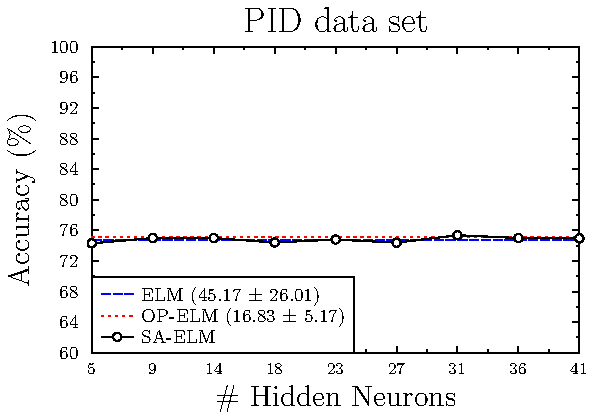
\includegraphics[width=\textwidth]{pid}
        \caption{Base de dados PID}
        \label{fig:pid}
    \end{subfigure}
    ~ 
    \begin{subfigure}[b]{0.45\textwidth}
        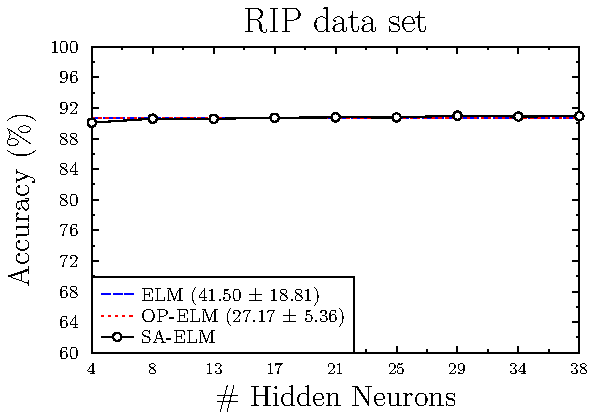
\includegraphics[width=\textwidth]{rip}
        \caption{Base de dados RIP}
        \label{fig:rip}
    \end{subfigure}
    \caption{Exemplo de gráfico}\label{fig:animals}
\end{figure}
% ------
\lipsum[1] 			% Capitulo de exemplo

% ----------------------------------------------------------
% Finaliza a parte no bookmark do PDF
% para que se inicie o bookmark na raiz
% e adiciona espaço de parte no Sumário
% ----------------------------------------------------------
\phantompart

% ---
% Conclusão
% ---
\chapter{Conclusão}
% ---

\lipsum[31-33] 				% Capítulo de introdução

% ----------------------------------------------------------
% ELEMENTOS PÓS-TEXTUAIS
% ----------------------------------------------------------
\postextual
% ----------------------------------------------------------

% ----------------------------------------------------------
% Referências bibliográficas
% ----------------------------------------------------------
\bibliography{referencias}

% ----------------------------------------------------------
% Glossário
% ----------------------------------------------------------
%
% Consulte o manual da classe abntex2 para orientações sobre o glossário.
%
%\glossary

% ----------------------------------------------------------
% Apêndices
% ----------------------------------------------------------

% ---
% Inicia os apêndices
% ---
\begin{apendicesenv}

% Imprime uma página indicando o início dos apêndices
\partapendices
% Insere os apêndices
% ----------------------------------------------------------
\chapter{Instalação de ambiente de desenvolvimento no Windows}
\label{ap:instalacao-env-windows}
% ----------------------------------------------------------
\lipsum[55-57]
\chapter{Quisque libero justo}
% ----------------------------------------------------------

\lipsum[50]
%\include{apendices/apendice-c}
%\include{apendices/apendice-d}




\end{apendicesenv}
% ---


% ----------------------------------------------------------
% Anexos
% ----------------------------------------------------------

% ---
% Inicia os anexos
% ---
\begin{anexosenv}

% Imprime uma página indicando o início dos anexos
\partanexos
% Insere os anexos
\chapter{Morbi ultrices rutrum lorem.}
% ---
\lipsum[30]

\chapter{Cras non urna sed feugiat cum sociis natoque penatibus et magnis dis
parturient montes nascetur ridiculus mus}
% ---

\lipsum[31]
%\include{anexos/anexo-c}
%\include{anexos/anexo-d}

\end{anexosenv}

%---------------------------------------------------------------------
% INDICE REMISSIVO
%---------------------------------------------------------------------
\phantompart
\printindex
%---------------------------------------------------------------------

\end{document}
